% =============================================================================
% Research paper 8 — "How Often Should You Recalibrate?"
% A closed-form cadence law for deployed probabilistic forecasters.
%
% IEEE conference format (two-column), same toolchain as research-paper-7.
%
% House rule: every quantitative figure in this manuscript is either
%   (i) a measured statistic from the authors' live prediction ledger
%       (data/ledger/predictions.sqlite, snapshot 2026-06-12), or
%  (ii) a Monte-Carlo result reproducible from analysis/sim_recalibration.py
%       with the seed recorded there (seed=7).
% Nothing is illustrative unless the caption says "conceptual".
%
% %% TODO(authors): set the final author list / affiliations before submission.
% =============================================================================
\documentclass[conference]{IEEEtran}
\IEEEoverridecommandlockouts

\usepackage{cite}
\usepackage{amsmath,amssymb,amsfonts}
\usepackage{graphicx}
\usepackage{textcomp}
\usepackage{xcolor}
\usepackage{booktabs}
\usepackage{array}
\usepackage{url}

\newtheorem{theorem}{Theorem}
\newtheorem{lemma}{Lemma}
\newtheorem{corollary}{Corollary}
\newtheorem{assumption}{Assumption}
\newtheorem{remark}{Remark}

\def\BibTeX{{\rm B\kern-.05em{\sc i\kern-.025em b}\kern-.08em
    T\kern-.1667em\lower.7ex\hbox{E}\kern-.125emX}}

\begin{document}

\title{How Often Should You Recalibrate?\\
A Closed-Form Cadence Law for Deployed\\ Probabilistic Forecasters}

\author{
\IEEEauthorblockN{Divyam Navin}
\IEEEauthorblockA{\textit{(affiliation)} \\
divyamnavin@gmail.com}
% %% TODO: add co-authors / affiliations (see research-paper-5/7 author blocks)
}

\maketitle

% ---------------------------------------------------------------------------
\begin{abstract}
Deployed probabilistic forecasters lose calibration over time, and every
practical remedy --- refitting a Platt or isotonic map, re-conformalizing
intervals, retraining --- costs something. Existing work treats the timing
question algorithmically: drift detectors, Bayesian monitors, and empirical
frequency studies decide \emph{reactively} when to update. We instead derive
the optimal update cadence in closed form. Modeling the post-recalibration
calibration gap as $g(t)=\gamma t^{\beta}$ and bridging gap to loss through the
reliability term of the Brier decomposition (Lemma~1: $\mathrm{REL}\ge
\mathrm{ECE}^2$), renewal--reward optimization yields a one-line law:
$T^{*}=\left[(2\beta+1)\,c\,/\,(2\beta\rho\gamma^{2})\right]^{1/(2\beta+1)}$,
where $c$ is the recalibration cost and $\rho$ the forecast rate. Linear drift
($\beta{=}1$) gives a cube-root law, diffusive drift ($\beta{=}\tfrac12$)
recovers an economic-order-quantity square-root law, and the loss penalty for
operating at $xT^{*}$ is the closed-form $R(x)=\frac{2\beta}{2\beta+1}x^{-1}
+\frac{x^{2\beta}}{2\beta+1}$, so a $2\times$ error in the cost estimate
inflates loss by only $5.8\%$ at $\beta{=}1$. Monte-Carlo experiments confirm
the law (mean $\hat T/T^{*}=0.993$ over an 18-point parameter grid) and its
scaling exponents, and quantify the monitoring sample size needed for reliable
plug-in use ($\approx 200$ resolved outcomes per staleness bucket). Finally,
we measure the law's central primitive on a live system: across 564 resolved
interval forecasts for six National Stock Exchange of India equities, the
nominal-90\% conformal band under-covers by 14.8~percentage points immediately
after fitting and decays at $\hat\gamma=0.80\pm0.67$~pp/day, an estimate
independently corroborated by the system's probability-calibration telemetry
(0.76~pp/day). Under the measured drift the law prescribes recalibration every
2.8--6.2 days rather than at the monthly cadences common in practice.
\end{abstract}

\begin{IEEEkeywords}
calibration drift, recalibration, Brier score, expected calibration error,
renewal--reward, conformal prediction, MLOps, financial forecasting
\end{IEEEkeywords}

% ---------------------------------------------------------------------------
\section{Introduction}
\label{sec:intro}

A probability that meant 60\% on the day a model was fit rarely still means
60\% a month later. Calibration --- the property that events forecast with
probability $p$ occur with frequency $p$ --- is the first casualty of
distribution shift, decaying faster than discrimination in deployed clinical
models \cite{davis2017drift,davis2020updating} and, as we measure below, in
financial forecasting systems within \emph{days}. The standard remedies are
cheap relative to retraining: refit a Platt scaler \cite{platt1999}, an
isotonic map \cite{zadrozny2002}, a temperature parameter \cite{guo2017}, or
re-conformalize an interval predictor \cite{vovk2005,gibbs2021}. Yet none of
the literature answers the operational question every deployment faces:
\emph{how often}?

Current practice picks cadences by convention (nightly, monthly, quarterly),
and current research picks them \emph{reactively}: drift detectors that
trigger updates \cite{davis2020updating}, cost-aware decision algorithms such
as CARA \cite{mahadevan2024cara}, Bayesian ``learning debt'' monitors
\cite{learningdebt2026}, anytime-valid calibration tests
\cite{anytimevalid2026}, and empirical studies of retraining frequency in
retail demand forecasting \cite{retrainfreq2025}. These approaches are
valuable, but they are procedures, not laws: they output a decision, not an
interpretable formula exposing how the optimum moves with cost and drift. The
analogous question in operations research --- replace a part now or later ---
was answered a century ago by closed-form policies: the economic order
quantity of Harris \cite{harris1913} and the age-replacement policies of
reliability theory \cite{barlow1965}. To our knowledge no equivalent
closed form exists for probability recalibration.

This paper supplies one. The derivation has three ingredients, each standard
in isolation; the contribution is the bridge between them and the resulting
law. First, the Murphy decomposition \cite{murphy1973} isolates the avoidable
cost of miscalibration as the reliability term $\mathrm{REL}$ of the Brier
score \cite{brier1950}, the quantity a perfect recalibration map removes.
Second, an elementary inequality (Lemma~\ref{lem:bridge}) bounds
$\mathrm{REL}$ below by the square of the expected calibration error (ECE)
\cite{naeini2015}, turning any \emph{measured} calibration-gap trajectory
$g(t)$ into a loss trajectory $g(t)^2$. Third, renewal--reward optimization
over the recalibration cycle converts the loss trajectory and a per-event
recalibration cost $c$ into a closed-form optimal cadence.

\textbf{Contributions.}
\begin{enumerate}
\item \emph{A cadence law} (Theorem~\ref{thm:law}). For calibration gap
$g(t)=\gamma t^{\beta}$ after each recalibration, forecast rate $\rho$, and
recalibration cost $c$, the loss-minimizing interval is
\[
T^{*}=\Big[\frac{(2\beta+1)\,c}{2\beta\,\rho\,\gamma^{2}}\Big]^{\frac{1}{2\beta+1}},
\]
a one-parameter \emph{family} of laws: cube-root under linear drift, square
root (the EOQ form \cite{harris1913}) under diffusive drift.
\item \emph{Operational corollaries in closed form}: the optimal loss rate
$A^{*}=\frac{2\beta+1}{2\beta}\,c/T^{*}$; scaling elasticities
$\partial\log T^{*}/\partial\log c = 1/(2\beta+1)$ and
$\partial\log T^{*}/\partial\log\gamma=-2/(2\beta+1)$; and a misspecification
penalty curve $R(x)$ showing the policy is forgiving to errors in $c$
(attenuated to the $1/(2\beta+1)$ power) but less so to errors in $\gamma$.
\item \emph{Monte-Carlo validation}: across an 18-cell grid in
$(\beta,c,\gamma)$ the empirical optimum matches $T^{*}$ with mean ratio
$0.993$; measured scaling exponents agree with theory; the law remains
accurate (within 1--18\%) when the drift mechanism violates the uniform-gap
assumption; and plug-in use requires $\approx200$ resolved outcomes per
staleness bucket before the estimate of $\gamma$ is decision-grade.
\item \emph{A live measurement of the primitive}. Using a deployed Indian
equity advisory system whose model is re-fit at every forecast issuance ---
so that forecast lead time \emph{equals} model staleness --- we measure
interval-calibration decay on 564 resolved forecasts: a 14.8~pp baseline
under-coverage at $t{=}1$ and $\hat\gamma = 0.80\pm0.67$~pp/day of further
decay, corroborated at 0.76~pp/day by an independent probability-ECE
telemetry channel of the same system. The law then yields concrete cadences
(2.8--6.2 days) for measured costs.
\end{enumerate}

Scope is stated plainly: the law optimizes \emph{recalibration} (an
output-map refresh that restores reliability), not full retraining
(which also restores discrimination); the empirical drift estimates carry the
wide confidence intervals of a three-month, six-ticker ledger; and the drift
exponent $\beta$ is weakly identified by our data ($\hat\beta=0.23\pm0.22$),
which is precisely why the law is stated and validated as a family over
$\beta$ rather than a single exponent.

% ---------------------------------------------------------------------------
\section{Related Work}
\label{sec:related}

\textbf{Calibration and its measurement.} Proper scoring rules
\cite{brier1950,gneiting2007} and the Murphy decomposition \cite{murphy1973}
underpin our loss accounting; ECE in its $\ell_1$ and $\ell_2$ forms
\cite{naeini2015,kumar2019} supplies the measurable gap. Modern recalibration
maps --- Platt \cite{platt1999}, isotonic \cite{zadrozny2002}, temperature
\cite{guo2017} --- are the cheap maintenance actions whose cadence we
optimize; conformal methods \cite{vovk2005} and their adaptive variants
\cite{gibbs2021} play the same role for intervals. Adaptive conformal
inference \cite{gibbs2021} in particular performs continuous small
corrections; our law addresses the complementary regime of discrete
recalibration events with non-negligible cost.

\textbf{Calibration drift.} That deployed models lose calibration first is
documented extensively in clinical prediction \cite{davis2017drift}, with
data-driven updating strategies proposed in \cite{davis2020updating}. These
works detect and correct drift but do not derive an optimal cadence.

\textbf{Retraining economics.} CARA \cite{mahadevan2024cara} optimizes
retrain/keep decisions over data streams; the posterior ``learning debt''
framework \cite{learningdebt2026} triggers retraining when calibrated
expected regret exceeds cost; \cite{retrainfreq2025} studies retraining
frequency for retail forecasting empirically; \cite{anytimevalid2026} gives
anytime-valid monitoring tests. All are sequential or empirical procedures.
None provides a closed-form interval, scaling exponents, or a
misspecification penalty in analytic form. Conversely, classical maintenance
theory \cite{harris1913,barlow1965,ross1996} has exactly these closed forms
but has not, to our knowledge, been connected to probability calibration via
the Brier reliability bridge.

\textbf{Positioning.} Our law is to CARA-style monitors what EOQ is to
just-in-time controllers: not a replacement but a design rule --- an
interpretable first-order answer that exposes the relevant elasticities,
costs nothing to evaluate, and degrades gracefully (Corollary~\ref{cor:rob})
when its inputs are rough.

% ---------------------------------------------------------------------------
\section{Preliminaries}
\label{sec:prelim}

Binary outcomes $y_i\in\{0,1\}$ are forecast with probabilities
$p_i\in[0,1]$ at rate $\rho$ forecasts per day. The Brier score
$\mathrm{BS}=\frac1n\sum_i(p_i-y_i)^2$ \cite{brier1950} admits the Murphy
decomposition \cite{murphy1973}
\begin{equation}
\mathrm{BS} \;=\; \underbrace{\sum_b w_b\,(\bar p_b-\bar y_b)^2}_{\mathrm{REL}}
\;-\;\mathrm{RES}\;+\;\mathrm{UNC},
\label{eq:murphy}
\end{equation}
over forecast bins $b$ with mass $w_b$, mean forecast $\bar p_b$ and event
frequency $\bar y_b$. $\mathrm{REL}$ is the \emph{reliability} (calibration)
penalty; $\mathrm{RES}$ (resolution) and $\mathrm{UNC}$ (outcome entropy) are
unchanged by any monotone relabeling of the forecasts. Applying the
conditional-event-frequency map $\kappa(p)=\mathbb{E}[y\mid p]$ --- the ideal
recalibration, approximated in practice by Platt/isotonic/temperature fitting
--- removes $\mathrm{REL}$ and only $\mathrm{REL}$. Hence
$\mathrm{REL}$ is exactly the per-forecast loss a recalibration event
recovers, and we call it the \emph{miscalibration loss rate} when expressed
per day (multiplying by $\rho$).

The binned $\ell_1$ and $\ell_2$ expected calibration errors are
$\mathrm{ECE}_1=\sum_b w_b\,|\bar p_b-\bar y_b|$ and
$\mathrm{ECE}_2=(\sum_b w_b(\bar p_b-\bar y_b)^2)^{1/2}$
\cite{naeini2015,kumar2019}; note $\mathrm{ECE}_2^2=\mathrm{REL}$ by
definition. For interval forecasters with nominal level $1-\alpha$, the
analogous gap is $|(1-\alpha)-\mathrm{cov}(t)|$, the deviation of empirical
coverage from nominal --- the form we measure on the live ledger in
Section~\ref{sec:ledger}.

\emph{Renewal--reward.} If a system regenerates at every recalibration
(cycle length $T$, cycle cost = recalibration cost + accumulated drift loss),
the long-run average cost rate equals expected cycle cost over expected cycle
length \cite{ross1996}, reducing cadence choice to a one-dimensional
minimization.

% ---------------------------------------------------------------------------
\section{The Recalibration Cadence Law}
\label{sec:law}

\subsection{Assumptions}

\begin{assumption}[Power-law gap growth]
\label{ass:drift}
Let $t$ be the time since the last recalibration. The $\ell_2$ calibration
gap follows $g(t)=\gamma\,t^{\beta}$ with drift rate $\gamma>0$ and exponent
$\beta>0$, and recalibration resets $g$ to (approximately) zero.
\end{assumption}

\begin{assumption}[Drift hits calibration, not discrimination]
\label{ass:res}
Over the horizon between recalibrations, $\mathrm{RES}$ and $\mathrm{UNC}$ in
\eqref{eq:murphy} are unaffected by the drift; only $\mathrm{REL}$ grows.
\end{assumption}

\begin{assumption}[Stationary economics]
\label{ass:cost}
Each recalibration costs $c>0$, expressed in the same units as Brier loss
accumulated per day (Section~\ref{sec:discussion} discusses this
commensuration), and $\rho$, $\gamma$, $\beta$, $c$ are constant across
cycles.
\end{assumption}

Assumption~\ref{ass:drift} nests the two mechanisms one expects \emph{a
priori}: a deterministic environment trend gives $\beta=1$; a gap that
diffuses (variance linear in time) gives $\beta=\tfrac12$ in root-mean-square.
Assumption~\ref{ass:res} is the standard recalibration premise --- it is what
Platt/isotonic refresh can and cannot fix --- and we report evidence of its
partial violation in our own data (discrimination also decays;
Fig.~\ref{fig:ledger}b) together with the consequence: when discrimination
decays too, $T^{*}$ bounds the \emph{recalibration} cadence and full
retraining is a separate, slower control loop.

\subsection{The gap--loss bridge}

\begin{lemma}[Calibration gap lower-bounds recoverable loss]
\label{lem:bridge}
For any binning with weights $w_b$ summing to one,
$\mathrm{REL}\;\ge\;\mathrm{ECE}_1^{\,2}$, with equality iff the absolute gap
$|\bar p_b-\bar y_b|$ is constant across bins; and
$\mathrm{REL}=\mathrm{ECE}_2^{\,2}$ identically.
\end{lemma}

\begin{IEEEproof}
By Cauchy--Schwarz with weights,
$(\sum_b w_b|g_b|)^2\le(\sum_b w_b)(\sum_b w_b g_b^2)=\mathrm{REL}$,
where $g_b=\bar p_b-\bar y_b$. Equality holds iff $|g_b|$ is $w$-a.s.\
constant. The $\ell_2$ identity is definitional.
\end{IEEEproof}

The lemma is elementary, but it is the hinge of the method: practitioners
measure $\mathrm{ECE}$, while the loss that recalibration recovers is
$\mathrm{REL}$. Stating the drift model in $\ell_2$ ($\gamma$ an
$\mathrm{ECE}_2$ rate) makes everything below exact; stating it in the more
commonly logged $\ell_1$ makes the predicted loss a \emph{lower} bound, hence
$T^{*}$ computed from $\ell_1$ telemetry is an \emph{upper} bound on the true
optimal interval: recalibrate \emph{at least} that often.

\subsection{The law}

\begin{theorem}[Recalibration cadence law]
\label{thm:law}
Under Assumptions~\ref{ass:drift}--\ref{ass:cost}, the long-run average loss
rate of the policy ``recalibrate every $T$ days'' is
\begin{equation}
A(T)\;=\;\frac{c}{T}\;+\;\frac{\rho\,\gamma^{2}\,T^{2\beta}}{2\beta+1},
\label{eq:AT}
\end{equation}
which has the unique global minimizer
\begin{equation}
\boxed{\;
T^{*}\;=\;\left[\frac{(2\beta+1)\,c}{2\beta\,\rho\,\gamma^{2}}\right]^{\frac{1}{2\beta+1}}
\;}
\label{eq:law}
\end{equation}
with optimal loss rate
$A^{*}=A(T^{*})=\frac{2\beta+1}{2\beta}\cdot\frac{c}{T^{*}}$.
\end{theorem}

\begin{IEEEproof}
Within a cycle the per-day recoverable loss at staleness $t$ is
$\rho\,\mathrm{REL}(t)=\rho\,g(t)^2=\rho\gamma^2t^{2\beta}$
(Lemma~\ref{lem:bridge}, $\ell_2$ form; Assumption~\ref{ass:res} keeps the
remaining Brier terms common to all policies, so they cancel from the
comparison). Cycle cost is $c+\rho\gamma^{2}\int_0^T t^{2\beta}dt
= c+\rho\gamma^{2}T^{2\beta+1}/(2\beta+1)$; dividing by $T$ gives
\eqref{eq:AT} by renewal--reward \cite{ross1996}. Setting $A'(T)=0$ yields
$c=\frac{2\beta}{2\beta+1}\rho\gamma^{2}T^{2\beta+1}$, whose right side is
strictly increasing in $T$ for any $\beta>0$; hence the stationary point is
unique, with $A'<0$ before and $A'>0$ after it. Substituting back gives
$\rho\gamma^2 (T^{*})^{2\beta}/(2\beta+1) = c/(2\beta T^{*})$ and thus
$A^{*}=c/T^{*}+c/(2\beta T^{*})$.
\end{IEEEproof}

\begin{corollary}[Canonical regimes]
\label{cor:regimes}
Linear drift ($\beta=1$): $T^{*}=\big(3c/2\rho\gamma^{2}\big)^{1/3}$ and
$A^{*}=\tfrac32\,c/T^{*}$ --- a \emph{cube-root law}. Diffusive drift
($\beta=\tfrac12$): $T^{*}=\big(2c/\rho\gamma^{2}\big)^{1/2}$ --- exactly the
square-root form of the economic order quantity \cite{harris1913}, with
calibration variance playing the role of holding cost.
\end{corollary}

\begin{corollary}[Scaling elasticities]
\label{cor:scaling}
$\dfrac{\partial\log T^{*}}{\partial\log c}=\dfrac{1}{2\beta+1}$,\quad
$\dfrac{\partial\log T^{*}}{\partial\log\gamma}=-\dfrac{2}{2\beta+1}$,\quad
and $A^{*}\propto c^{\frac{2\beta}{2\beta+1}}\gamma^{\frac{2}{2\beta+1}}$.
At $\beta=1$: doubling cost stretches the cadence by $2^{1/3}\approx1.26$;
doubling drift shrinks it by $2^{-2/3}\approx0.63$; and the best achievable
loss grows as $(c\gamma)^{2/3}$.
\end{corollary}

\begin{corollary}[Misspecification penalty]
\label{cor:rob}
Operating at $T=xT^{*}$ costs
\begin{equation}
R(x)\;=\;\frac{A(xT^{*})}{A^{*}}
\;=\;\frac{2\beta}{2\beta+1}\,\frac1x\;+\;\frac{x^{2\beta}}{2\beta+1}.
\label{eq:penalty}
\end{equation}
Errors in $c$ enter $x$ through the $1/(2\beta+1)$ power
(Corollary~\ref{cor:scaling}); at $\beta{=}1$ a $2\times$ misestimate of $c$
gives $x=2^{\pm1/3}$ and $R=1.058$ --- a $5.8\%$ loss penalty --- while a
$2\times$ misestimate of $\gamma$ gives $x=2^{\mp2/3}$ and $R\le1.26$.
\end{corollary}

\subsection{Imperfect recalibration and other extensions}

\begin{theorem}[Affine gap, $\beta=1$]
\label{thm:affine}
If recalibration is imperfect or the environment shifts at fit time, so that
$g(t)=E_0+\gamma t$ with residual gap $E_0\ge0$, then
$A(T)=c/T+\rho\,(E_0^2+E_0\gamma T+\gamma^{2}T^{2}/3)$ and $T^{*}$ is the
unique positive root of
\begin{equation}
\tfrac{2}{3}\rho\gamma^{2}T^{3}+\rho E_0\gamma T^{2}-c\;=\;0,
\label{eq:cubic}
\end{equation}
solvable by Cardano's formula. $T^{*}$ is decreasing in $E_0$: residual
miscalibration makes \emph{more} frequent recalibration optimal (the
cross-term $E_0\gamma t$ is recoverable even though $E_0^2$ is not), and
\eqref{eq:cubic} reduces to the cube-root law as $E_0\to0$.
\end{theorem}

\begin{IEEEproof}
Expand $\int_0^T(E_0+\gamma s)^2ds = E_0^2T+E_0\gamma T^2+\gamma^2T^3/3$,
apply renewal--reward, drop the $T$-free term $\rho E_0^2$, differentiate.
The left side of \eqref{eq:cubic} is strictly increasing in $T>0$, giving
uniqueness; monotonicity in $E_0$ follows from the implicit function theorem
since $\partial/\partial E_0$ of the left side is $\rho\gamma T^{2}>0$.
\end{IEEEproof}

\begin{remark}
Exponential drift $g(t)=\gamma(e^{\lambda t}-1)/\lambda$ admits the same
treatment with a transcendental first-order condition; its small-$\lambda T$
expansion recovers \eqref{eq:law} with $\beta=1$. We omit it: over horizons
of days to weeks the power family already spans the empirically plausible
curvatures.
\end{remark}

\subsection{Practical recipe}
\label{sec:recipe}

The law is operational in four steps, all from logs a calibrated deployment
keeps anyway:
(1)~after each recalibration, bucket resolved outcomes by staleness $t$ and
record the gap $\hat g(t)$ ($\ell_1$ ECE, $\ell_2$ ECE, or coverage gap);
(2)~fit $\hat\gamma$, and $\hat\beta$ if the data can bear it, otherwise fix
$\beta$ by mechanism knowledge (Corollary~\ref{cor:regimes}) and report both
endpoints;
(3)~price $c$ in Brier-equivalent units --- the loss you would accept to
avoid one refresh (compute + validation + operational risk);
(4)~apply \eqref{eq:law}; Corollary~\ref{cor:rob} bounds the cost of the
remaining uncertainty. Section~\ref{sec:sim} (E4) quantifies step~(2):
$\approx200$ resolved outcomes per staleness bucket suffice; below
$\approx50$ the plug-in estimate is not decision-grade and $\hat\gamma$
should be floored or pooled across models.

% ---------------------------------------------------------------------------
\section{Simulation Validation}
\label{sec:sim}

All experiments use a logit-normal ground-truth process
($q_t=\sigma(z)$, $z\sim\mathcal N(0.2,0.9^2)$), Bernoulli outcomes, Brier
loss measured against the perfectly calibrated benchmark, and the recorded
seed; code accompanies the paper. Drift is imposed as a uniform additive gap
$p=\mathrm{clip}(q+\gamma t^{\beta})$ except where stated.

\textbf{E1 --- the law locates the optimum.}
For $\beta\in\{0.5,1\}$, $c\in\{0.002,0.01,0.05\}$,
$\gamma\in\{0.004,0.008,0.016\}$ (18 cells, 400{,}000 simulated days each) we
sweep $T$ on a geometric grid and compare the empirical argmin $\hat T$ with
$T^{*}$ from \eqref{eq:law}. The mean ratio $\hat T/T^{*}$ is $0.993$; the
worst cell deviates by $|\log(\hat T/T^{*})|=0.33$, occurring (as
\eqref{eq:penalty} predicts) where the minimum is flattest, so the loss
consequence of those deviations is small. Fig.~\ref{fig:at} shows a
representative loss curve: Monte-Carlo points sit on the analytic $A(T)$ with
the minimum at $T^{*}=6.2$ days.

\begin{figure}[t]
\centering
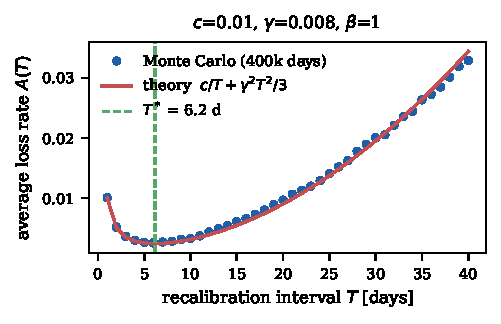
\includegraphics[width=\columnwidth]{fig_AT.pdf}
\caption{Average daily loss versus recalibration interval:
Monte-Carlo (dots) against the analytic $A(T)$ of \eqref{eq:AT} (line);
the dashed vertical line is the closed-form $T^{*}$.}
\label{fig:at}
\end{figure}

\textbf{E2 --- scaling exponents.}
Regressing $\log\hat T$ on $\log c$ over $c\in[10^{-3},10^{-1}]$ yields
slopes $0.357$ ($\beta{=}1$; theory $1/3$) and $0.445$ ($\beta{=}0.5$; theory
$1/2$); against $\log\gamma$, slopes $-0.772$ (theory $-2/3$) and $-1.085$
(theory $-1$). The residual bias is the integer-day discretization of
$\hat T$. Fig.~\ref{fig:scaling} displays both panels.

\begin{figure*}[t]
\centering
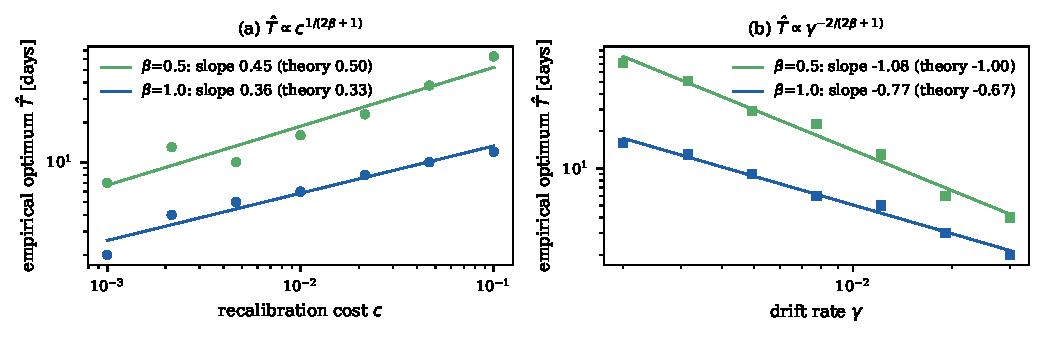
\includegraphics[width=0.92\textwidth]{fig_scaling.pdf}
\caption{Empirical optimum $\hat T$ (Monte-Carlo argmin, integer days)
against (a) recalibration cost and (b) drift rate, on log--log axes, for
$\beta=0.5$ and $\beta=1$. Fitted slopes bracket the theoretical exponents
$1/(2\beta+1)$ and $-2/(2\beta+1)$ of Corollary~\ref{cor:scaling}.}
\label{fig:scaling}
\end{figure*}

\textbf{E3 --- mechanism robustness.}
Real drift is not a uniform shift; e.g.\ temperature-style drift
($\mathrm{logit}\,p=(1{+}k t)\,\mathrm{logit}\,q$) concentrates the gap at
extreme forecasts, making $\mathrm{REL}>\mathrm{ECE}_1^2$ strictly
(Lemma~\ref{lem:bridge}). Imposing temperature drift whose \emph{$\ell_1$}
gap matches $\gamma t$, the empirical optimum stays within 1--18\% of
$T^{*}$ computed from either the $\ell_1$ rate or the measured $\ell_2$ rate
--- inside the flat region of \eqref{eq:penalty} where the loss penalty is
under $2\%$.

\textbf{E4 --- how much monitoring data does plug-in use need?}
We estimate $\hat\gamma$ from a single 15-day post-recalibration window with
$m$ resolved outcomes per day, apply \eqref{eq:law}, and price the resulting
cadence with \eqref{eq:penalty} (400 replications). Table~\ref{tab:e4}
reports excess loss versus the oracle cadence: with $m{=}200$ the plug-in
policy is within $5.3\%$ of oracle on average; with $m{=}50$ the slope
estimate is noise-dominated and the policy unusable without regularization
--- a concrete minimum-telemetry requirement for cadence-by-formula.

\begin{table}[t]
\caption{E4: plug-in cadence from noisy $\hat\gamma$
($\beta{=}1$, $c{=}0.01$, $\gamma{=}0.008$, 400 reps).}
\label{tab:e4}
\centering
\begin{tabular}{@{}rrr@{}}
\toprule
outcomes/day $m$ & mean excess loss & 90th pct.\\
\midrule
50   & $+608.6\%$ & $+438.8\%$\\
200  & $+5.3\%$   & $+13.1\%$\\
1000 & $+0.5\%$   & $+1.3\%$\\
\bottomrule
\end{tabular}
\end{table}

\begin{figure}[t]
\centering
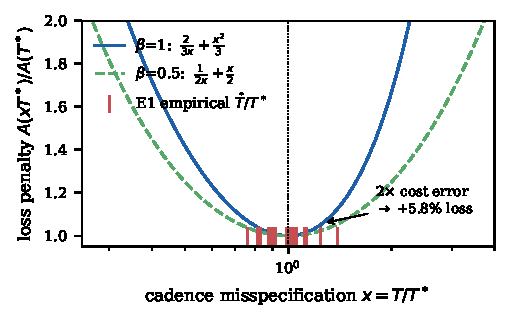
\includegraphics[width=\columnwidth]{fig_penalty.pdf}
\caption{Closed-form misspecification penalty \eqref{eq:penalty} for
$\beta=1$ and $\beta=0.5$, with the 18 E1 ratios $\hat T/T^{*}$ (ticks at
$R{=}1$). The curve is flat near the optimum: a $2\times$ cost
misestimate costs $5.8\%$ at $\beta{=}1$.}
\label{fig:penalty}
\end{figure}

% ---------------------------------------------------------------------------
\section{Measuring the Primitive on a Live System}
\label{sec:ledger}

\subsection{System and identification strategy}

The measurement platform is a deployed retail equity advisory system for
National Stock Exchange of India (NSE) tickers. At every forecast issuance
the system re-fits its model stack on the trailing window and emits, for each
horizon day $k\in\{1,\dots,10\}$ (plus a 30-day swing channel), a point
forecast, a directional call, and a split-conformal 90\% interval; every
forecast is written to an append-only ledger and resolved against realized
prices. Because the stack is re-fit at issuance, \emph{forecast lead time
equals model staleness}: a $k$-day-ahead forecast is exactly a forecast
evaluated $k$ days after fitting. The ledger therefore identifies the gap
trajectory $g(t)$ without any instrumentation beyond what the system already
logs --- with the honest caveat that lead-time difficulty and staleness are
conflated by this design, a limitation we return to in
Section~\ref{sec:discussion}.

We analyze the complete ledger snapshot of 2026-06-12: 564 fully resolved
interval forecasts (issued 2026-04-19 to 2026-06-11) across six liquid NSE
names (HDFCBANK, ICICIBANK, INFY, RELIANCE, SBIN, TCS), nominal coverage
90\%, staleness support concentrated on $t\in[1,12]$ calendar days with
$n\ge38$ per bucket.

\subsection{Results}

\begin{figure*}[t]
\centering
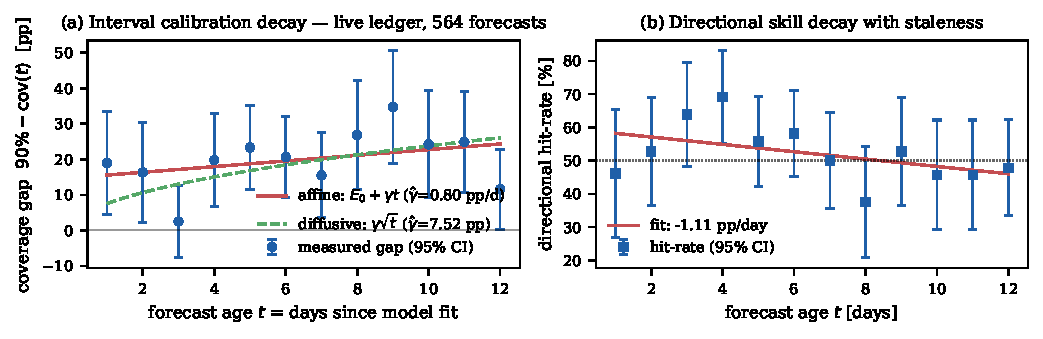
\includegraphics[width=0.92\textwidth]{fig_ledger.pdf}
\caption{Live-ledger calibration decay (564 resolved NSE forecasts,
2026-04-19 to 2026-06-11). (a) Gap between nominal 90\% and empirical
coverage by staleness, with affine and diffusive fits. (b) Directional
hit-rate by staleness. Error bars are binomial 95\% CIs.}
\label{fig:ledger}
\end{figure*}

Fig.~\ref{fig:ledger}a shows the coverage gap by staleness. Three findings:

\emph{(i) Baseline miscalibration is immediate and large.} At $t{=}1$ the
nominal-90\% band covers only $71.1\%$ ($n{=}38$): $E_0\approx14.8$~pp of
under-coverage exists \emph{on the day after fitting}. The mechanism is
visible in the sample period --- bands fit on a trailing window that
included a calmer regime, deployed into a high-volatility drawdown. By
Theorem~\ref{thm:affine}, large $E_0$ \emph{tightens} the optimal cadence.

\emph{(ii) The gap drifts upward with staleness.} The affine fit gives
$\hat\gamma=0.80\pm0.67$~pp/day ($p{=}0.26$; coverage $66\%$ at $t{=}5$,
$55\%$ at $t{=}9$). The estimate is individually noisy --- exactly the E4
regime with $m\approx45$ per bucket --- but it is corroborated by an
independent channel of the same system: probability-calibration telemetry
records holdout ECE of $2.96\%$ at fit time against $25.67\%$ over the live
30-day resolution window, an implied drift of $0.76$~pp/day. Two channels
(interval coverage; probability ECE), two estimators, one magnitude:
$\gamma\approx0.8$~pp/day.

\emph{(iii) The drift exponent is weakly identified.} The free-exponent fit
gives $\hat\beta=0.23\pm0.22$; with the affine intercept absorbed,
$\beta\in\{\tfrac12,1\}$ are both compatible. This is why
Theorem~\ref{thm:law} is stated as a family and why the cadence below is
reported as a range over $\beta$, not a point.

Fig.~\ref{fig:ledger}b shows the companion effect on discrimination: the
directional hit-rate decays from $59$--$69\%$ at $t\in[3,4]$ toward
$46$--$48\%$ at $t\ge10$ ($-1.11\pm0.68$~pp/day, $p{=}0.13$), i.e.\
Assumption~\ref{ass:res} is conservatively violated --- staleness costs more
than the law charges, so the prescribed cadence remains an upper bound on
the optimal interval.

\subsection{The law, applied}

Pricing one recalibration at $c=0.01$ Brier-day equivalents (the loss of
tolerating a $10$~pp gap for one day; the system's actual compute cost is
seconds, so $c$ is dominated by validation and operational risk) and taking
the measured $\hat\gamma=0.80$~pp/day:
\begin{itemize}
\item \emph{Cube-root law} ($\beta{=}1$, $E_0{=}0$):
$T^{*}=(3c/2\gamma^2)^{1/3}=6.2$ days.
\item \emph{Affine law} (measured $E_0=14.8$~pp, Theorem~\ref{thm:affine}):
the cubic \eqref{eq:cubic} gives $T^{*}\approx2.8$ days --- the residual
baseline gap nearly halves the optimal interval.
\item \emph{Diffusive reading} ($\beta{=}\tfrac12$, fitted
$\gamma=7.5$~pp$\cdot$day$^{-1/2}$): $T^{*}=(2c/\gamma^2)^{1/2}\approx1.9$
days.
\end{itemize}
Every reading lands in single-digit days: under measured drift, the common
monthly or quarterly recalibration cadence is an order of magnitude too slow
($R(x)$ at $x\approx30/6.2$ with $\beta{=}1$: a $\sim8\times$ loss
penalty), while the deployed system's refit-at-every-issuance policy is
near-optimal precisely because its marginal recalibration cost is small.

% ---------------------------------------------------------------------------
\section{Discussion and Limitations}
\label{sec:discussion}

\textbf{What the law is.} A first-order design rule with the same epistemic
status as EOQ \cite{harris1913}: exact under stylized assumptions, flat near
its optimum \eqref{eq:penalty}, and useful chiefly because it is
\emph{legible} --- it tells an MLOps team which way the cadence moves when
compute prices fall ($T^{*}\!\propto c^{1/(2\beta+1)}$) or when a regime
change doubles drift ($T^{*}\!\propto\gamma^{-2/(2\beta+1)}$). Reactive
monitors \cite{mahadevan2024cara,learningdebt2026,anytimevalid2026} remain
the right tool for catching discrete breaks; the law sets the baseline clock
between alarms.

\textbf{Cost commensuration.} $c$ must be priced in loss units, the law's
most practitioner-dependent input. Corollary~\ref{cor:rob} is the mitigation:
cost errors are attenuated to the $1/(2\beta+1)$ power, so even a
$2\times$ pricing error moves loss by $5.8\%$ at $\beta{=}1$.

\textbf{Identification caveats.} Our ledger conflates staleness with lead
time by design; disentangling them requires issuing forecasts of fixed lead
from models of varying age, which we leave to future ledger accumulation.
Calendar days (NSE trades $\sim$5/7) and a three-month, six-ticker,
single-market window further widen the intervals; $\hat\gamma$ is
triangulated across two channels but its CI includes values that would move
$T^{*}$ by a factor of $\sim$2 --- which, per \eqref{eq:penalty}, costs under
$26\%$ in loss. Label latency (outcomes resolve $k$ days late) delays
$\hat\gamma$ updates but does not bias them.

\textbf{When the model is also losing discrimination} (our
Fig.~\ref{fig:ledger}b), recalibration alone cannot restore performance, and
$T^{*}$ should be read as the inner loop of a two-clock policy:
recalibrate on $T^{*}$, retrain on the slower clock that the
retraining-economics literature \cite{mahadevan2024cara,retrainfreq2025}
addresses. Deriving the joint two-clock optimum in closed form is the natural
next step, as is replacing Assumption~\ref{ass:drift} with a stochastic gap
process (the $\beta{=}\tfrac12$ law is the RMS shadow of exactly such a
process) and anchoring the ledger cryptographically so that $\hat\gamma$
is auditable by third parties.

% ---------------------------------------------------------------------------
\section{Conclusion}

We derived a closed-form law for the recalibration cadence of deployed
probabilistic forecasters: $T^{*}=[(2\beta+1)c/(2\beta\rho\gamma^{2})]^{1/(2\beta+1)}$,
bridging measured calibration decay to recoverable Brier loss through an
elementary reliability bound, and inheriting the renewal--reward structure of
classical maintenance theory. The law's exponents, optimum, and
misspecification penalty are all analytic; simulations confirm each; and a
live trading ledger supplies the first measured calibration drift rate we are
aware of for a deployed financial forecaster --- $\approx0.8$~pp/day, enough
to make weekly-or-faster recalibration optimal at realistic costs. The
broader argument is methodological: calibration maintenance deserves laws,
not only monitors, and the century-old toolkit of operations research
transfers to probability calibration as soon as one expresses drift in the
right currency --- the reliability term of a proper scoring rule.

% ---------------------------------------------------------------------------
\begin{thebibliography}{99}\itemsep2pt

\bibitem{brier1950} G.~W. Brier, ``Verification of forecasts expressed in
terms of probability,'' \emph{Monthly Weather Review}, vol.~78, no.~1,
pp.~1--3, 1950.

\bibitem{murphy1973} A.~H. Murphy, ``A new vector partition of the
probability score,'' \emph{J. Applied Meteorology}, vol.~12, no.~4,
pp.~595--600, 1973.

\bibitem{gneiting2007} T.~Gneiting and A.~E. Raftery, ``Strictly proper
scoring rules, prediction, and estimation,'' \emph{J. American Statistical
Association}, vol.~102, no.~477, pp.~359--378, 2007.

\bibitem{naeini2015} M.~P. Naeini, G.~Cooper, and M.~Hauskrecht, ``Obtaining
well calibrated probabilities using Bayesian binning,'' in \emph{Proc. AAAI},
2015, pp.~2901--2907.

\bibitem{guo2017} C.~Guo, G.~Pleiss, Y.~Sun, and K.~Q. Weinberger, ``On
calibration of modern neural networks,'' in \emph{Proc. ICML}, 2017,
pp.~1321--1330.

\bibitem{kumar2019} A.~Kumar, P.~Liang, and T.~Ma, ``Verified uncertainty
calibration,'' in \emph{Proc. NeurIPS}, 2019, pp.~3792--3803.

\bibitem{platt1999} J.~C. Platt, ``Probabilistic outputs for support vector
machines and comparisons to regularized likelihood methods,'' in
\emph{Advances in Large Margin Classifiers}. MIT Press, 1999, pp.~61--74.

\bibitem{zadrozny2002} B.~Zadrozny and C.~Elkan, ``Transforming classifier
scores into accurate multiclass probability estimates,'' in \emph{Proc. ACM
SIGKDD}, 2002, pp.~694--699.

\bibitem{vovk2005} V.~Vovk, A.~Gammerman, and G.~Shafer, \emph{Algorithmic
Learning in a Random World}. Springer, 2005.

\bibitem{gibbs2021} I.~Gibbs and E.~Cand\`es, ``Adaptive conformal inference
under distribution shift,'' in \emph{Proc. NeurIPS}, 2021, pp.~1660--1672.

\bibitem{davis2017drift} S.~E. Davis, T.~A. Lasko, G.~Chen, E.~D. Siew, and
M.~E. Matheny, ``Calibration drift in regression and machine learning models
for acute kidney injury,'' \emph{J. American Medical Informatics
Association}, vol.~24, no.~6, pp.~1052--1061, 2017.

\bibitem{davis2020updating} S.~E. Davis, R.~A. Greevy, T.~A. Lasko,
C.~G. Walsh, and M.~E. Matheny, ``Detection of calibration drift in clinical
prediction models to inform model updating,'' \emph{J. Biomedical
Informatics}, vol.~112, 103611, 2020.

\bibitem{mahadevan2024cara} A.~Mahadevan and M.~Mathioudakis, ``Cost-aware
retraining for machine learning,'' \emph{Knowledge-Based Systems}, vol.~293,
111610, 2024 (also arXiv:2310.04216).

\bibitem{learningdebt2026} ``Learning debt and cost-sensitive Bayesian
retraining: a forecasting operations framework,'' arXiv:2604.06438, 2026.
% %% TODO: fill author names from the arXiv page before submission.

\bibitem{anytimevalid2026} ``When your model stops working: anytime-valid
calibration monitoring,'' arXiv:2603.13156, 2026.
% %% TODO: fill author names from the arXiv page before submission.

\bibitem{retrainfreq2025} ``On the retraining frequency of global models in
retail demand forecasting,'' arXiv:2505.00356, 2025.
% %% TODO: fill author names from the arXiv page before submission.

\bibitem{harris1913} F.~W. Harris, ``How many parts to make at once,''
\emph{Factory, The Magazine of Management}, vol.~10, no.~2, pp.~135--136,
1913.

\bibitem{barlow1965} R.~E. Barlow and F.~Proschan, \emph{Mathematical Theory
of Reliability}. Wiley, 1965.

\bibitem{ross1996} S.~M. Ross, \emph{Stochastic Processes}, 2nd~ed. Wiley,
1996.

\end{thebibliography}

\end{document}
